\documentclass{article}
\usepackage[english]{babel}
\usepackage[utf8x]{inputenc}
\usepackage[legalpaper, portrait, margin=1in]{geometry}
\usepackage{apacite}
\usepackage{algorithmic}
\usepackage{algorithm}
\usepackage{paralist}
\usepackage{tikz}

\title{Notes using Po-Mo models to detect hybridization/introgression}
\author{Mark T.~Holder}

\begin{document}
\maketitle

{\em The biological question:} We have an outgroup and three closely related ingroup taxa. Is there evidence that any pair of ingroup taxa have experienced introgression/hybridization since the most recent speciation event within the ingroup?

{\em The data:} We have sequence data from a few individuals of each species for a thousands of loci.  Some heterozygotes can be partially phased, but for the most part the data is unphased when individuals are heterozygous.

\section{Notes on a PoMo-based approach}
There are many methods for detecting introgression \cite{HibbinsHahn2021,HibbinsHahn2022} from ``phylogenomic'' data.
Coalescent-based approaches usually assume haplotype data.
This presents problems when phasing is difficult.

PoMo models (see \cite{schrempf2016reversible,borges2020consistency} and references there in) coarsen 
the data by ignoring haplotype structure and binning the frequency of polymorphisms into a few frequency categories.
However, they allow for efficient handling of very large datasets and provide many of the benefits that come from allowing 
species to be modelled as polymorphic for the duration of a branch in a species tree.

Current implementations would allow one to estimate rooted phylogenetic trees using PoMo models.
For the sake of simplicity we can consider the case of estimating a rooted quartet assuming a molecular clock for the mutational process and an equal rate of drift (constant and equal effective population sizes across all 4 species).

We will denote tip taxa with capital letters, $A$, $B$, $C$, and $D$.
If the rooted quartet species trees have the outgroup (taxon $D$) as sister to the 3 ingroup taxa, then there just three
possible species trees: $T_{AB}$, $T_{AC}$, and $T_{BC}$ where the subscripts denote the indices of the two ingroup
taxa that are sister to each other.
Each tree model also has 3 node height parameters for the ``sister'' ($S$) MRCA, the ``ingroup'' ($I$) MRCA and ``root'' ($\rho$) MRCA obeying the constraint that: $\tau_S < \tau_I < \tau_\rho$

Throughout the notes, we will consider the tree-backbone of the network to be $T_{AB}$ with a hybridization/introgression event between $B$ and $C$; See Figure \ref{fig:tree}.

\subsection{Proposed extension}
Can we calculate a likelihood for a phylogenetic network. 
The easiest case would be:
\begin{compactitem}
    \item Add a single network edge with between one of the sister taxa and the third ingroup taxon; as mentioned above, we will use $B$ and $C$ as th labels for these taxa.
    \item The edge (and the two hybridization parents) have height $\tau_H$ where $\tau_H < \tau_S$.
    \item There is a single unknown fraction $\phi$ of sites that have their frequencies affected by the hybridization.
    \item Ignoring linkage we can treat each site as independent with respect to this mixing parameter $\psi$
    \item There is a pair of fraction $\gamma_S$ and $\gamma_I$ that determine the post mixing frequency at each hybridized lineage immediately after the event as a weight in a weighted average between the 2 parental frequencies.
\end{compactitem}

\begin{figure}[htp]
\centering
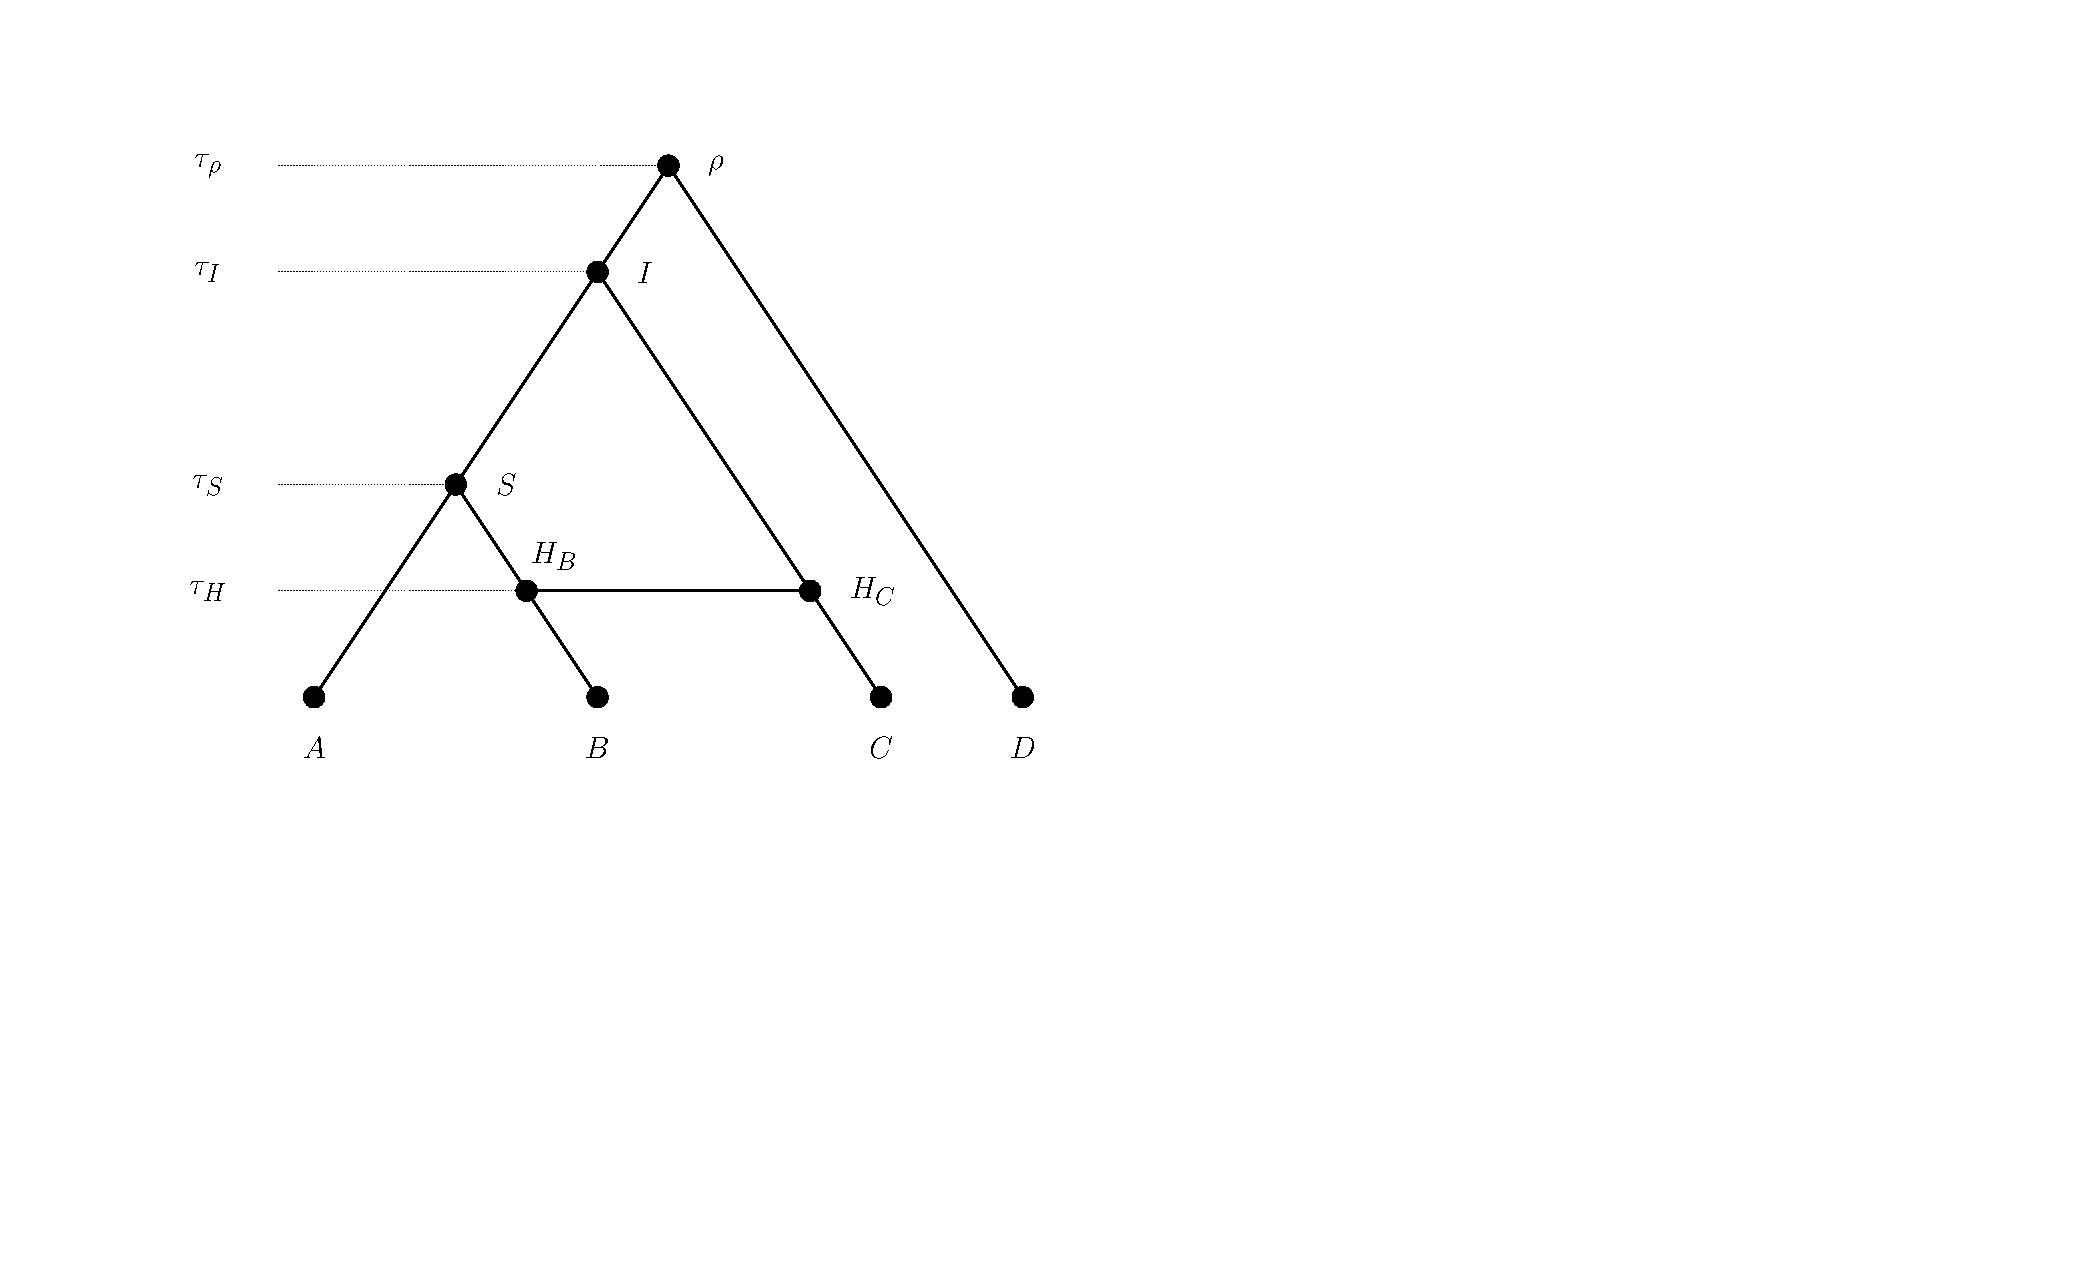
\includegraphics[scale=0.6]{figure1.pdf}
%\scalebox{0.3}{\begin{tikzpicture}[font=\Huge]
\coordinate  (root) at (11,16);
\coordinate [label=right:$\rho$] (rootlabel) at (12,16);
\coordinate (tipa) at (1,1);
\coordinate [label=below:$A$] (alabel) at (1,0);
\coordinate (tipb) at (9,1);
\coordinate [label=below:$B$] (blabel) at (9,0);
\coordinate (tipc) at (17,1);
\coordinate [label=below:$C$] (clabel) at (17,0);
\coordinate (tipd) at (21,1);
\coordinate [label=below:$D$] (dlabel) at (21,0);
\coordinate (sisters) at (5,7);
\coordinate [label=right:$S$] (slabel) at (6,7);
\coordinate (ingroup) at (9,13);
\coordinate [label=right:$I$] (ilabel) at (10,13);
\coordinate (hybsis) at (7,4);
\coordinate [label=right:$H_B$] (hblabel) at (7,5);
\coordinate (hybouter) at (15,4);
\coordinate [label=right:$H_C$] (hclabel) at (16,4);
\fill (root) circle (2ex);
\fill (tipa) circle (2ex);
\fill (tipb) circle (2ex);
\fill (tipc) circle (2ex);
\fill (tipd) circle (2ex);
\draw[ultra thick] [-] (root) -- (tipa) ;
\draw[ultra thick] [-] (root) -- (tipd);
\fill (sisters) circle (2ex);
\fill (ingroup) circle (2ex);
\draw[ultra thick] [-] (sisters) -- (tipb);
\draw[ultra thick] [-] (ingroup) -- (tipc);
\fill (hybsis) circle (2ex);
\fill (hybouter) circle (2ex);
\draw[ultra thick] [-] (hybsis) -- (hybouter);
\draw[dotted] [-] (0,4) -- (7,4);
\node[] at (-2,4) {$\tau_H$};
\draw[dotted] [-] (0,7) -- (5,7);
\node[] at (-2,7) {$\tau_S$};
\draw[dotted] [-] (0,13) -- (9,13);
\node[] at (-2,13) {$\tau_I$};
\draw[dotted] [-] (0,16) -- (11,16);
\node[] at (-2,16) {$\tau_\rho$};
\end{tikzpicture}

}
\caption{Depiction of tree with node and node depth parameter labeling used throughout these notes. We consider a rooted four-taxon tree with a single outgroup ($D$) and hybridization/introgression event between two non-sister taxa ($B$ and $C$) in the ingroup. The hybridization nodes are labeled with $H$ and with a $B$ or $C$ subscript indicating which tip they are a parent to. The internal tree-nodes are labelled $S$, $I$, and $\rho$ to denote the sister, ingroup and root, respectively.}
\label{fig:tree}
\end{figure}

\subsection{Algorithm}
\subsubsection{Overview}
Most of the calculations are the same as in PoMo.
To deal with the hybridization/introgression event, we introduce a partial likelihood arrays (PLA) immediately before and after the event; in other words rootward and tipward of $H_B$ and $H_C$.
We will use $\uparrow$ to denote the rootward side of a node and $\downarrow$ to denote the tipward side of a node.
The only transitions between the two are the result of the mixing (with probability $\phi$ and weighting $\gamma_S$ and $\gamma_I$ then binning into the PoMo frequency bins).


The root-ward PLA has the size that is the square of the PoMo state space, because we need to account for the joint events: the probability that the $H_{B\uparrow}$ is in state $i$ and $H_{C\uparrow}$ is in state $j$ in order to correctly calculate the probability of the data tipward of the hybridization event.
But this expanded state space only affects a few nodes (because our tree is small, and we recondense to the PoMo state space at node $I$.

\subsubsection{Notation}
Because all sites follow the same model the calculations described would be calculated for each data pattern.
Here we will elide the introduction of a dimension and indexing to refer to each data pattern, but in a real implementation the data structures would be arrays of the ones described below with an index for the site pattern.





\bibliographystyle{apacite}
\bibliography{pomorefs}


\end{document}


